\documentclass[conference]{IEEEtran}
\usepackage{graphicx} % Required for including graphics
\usepackage{amsmath} % For mathematical symbols
\usepackage{cite} % For citations


% IEEE Header and Footer
\pagestyle{plain}

\begin{document}

% Title page
\title{A 2.2V Analog Integrated Implementation of a Gaussian Mixture Model Classifier}
\author{
    \IEEEauthorblockN{Athanasios Liakopoulos}
    \IEEEauthorblockA{National Technical University of Athens, Greece\\
    School of Electrical and Computer Engineering\\
    \texttt{nassosliak@gmail.com}}
}
\maketitle

\begin{abstract}
This paper presents the design and implementation of a 2.2V analog Gaussian Mixture Model (GMM) classifier, a probabilistic model frequently employed in unsupervised learning tasks such as clustering and density estimation. The proposed analog classifier is composed of multiple Gaussian function circuits and a Winner-Take-All (WTA) circuit, offering modularity and scalability in terms of the number of classes and input dimensionality. The functionality and performance of the analog GMM classifier were validated through simulations conducted using the Cadence IC Suite. Additionally, a comparative analysis between the hardware implementation and its software counterpart is provided, utilizing the Breast Cancer dataset from the University of Wisconsin to demonstrate the efficacy of the analog approach.
\end{abstract}

\begin{IEEEkeywords}
Analog Integrated Implementation, Classifier, Gaussian Mixture Model
\end{IEEEkeywords}

\section{\textbf{Introduction}}
The exponential growth in data availability, coupled with significant advancements in computing hardware, has driven rapid progress in the fields of Machine Learning (ML) and Deep Learning (DL) \cite{panic2020gaussian}. 
Implementing machine learning (ML) techniques in production requires extensive data collection and a computationally intensive algorithmic inference process. Typically, this processing is carried out on high-cost hardware systems like data centers \cite{ALIMISIS2022105510}. Many of the machine learning (ML) applications require real-time processing, which creates challenges due to the impracticality of transferring large amounts of data between data acquisition systems and centralized data centers. Edge computing addresses this issue by integrating data acquisition and processing into the same device, thereby eliminating communication delays \cite{ALIMISIS2022105510}. This approach is particularly relevant to the emerging field of smart industries, where Internet of Things (IoT) applications can leverage ML models . A critical consideration for IoT systems is power efficiency , as devices must perform complex computations autonomously, often relying on battery power. This has driven the demand for extremely low power consumption and compact designs \cite{ALIMISIS2022105510}. As a result, recent years have seen a growing trend toward low-power, low-area hardware accelerators for IoT and ML applications, directly connected to smart sensors or systems .\\



Leveraging these developments, this paper presents the design and implementation of a fully analog integrated Gaussian Mixture Model (GMM) classifier. We begin by introducing the fundamental principles of the GMM classifier, covering both its mathematical foundation and hardware implementation. Following this, the primary building blocks of the classifier are analyzed in detail. Finally, we demonstrate the performance and capabilities of the low power hardware classifier in comparison to its software counterpart.

\section{\textbf{Analysis of the GMM Classifier}}
The Gaussian Mixture Model (GMM) is a probabilistic model that assumes that the data is generated from a mixture of several Gaussian distributions with unknown parameters. It is widely used in clustering, density estimation, and other unsupervised learning tasks.
In this approach, each class is individually modeled using a separate GMM for data clustering, independent of the other classes. The number of components (clusters) within each GMM is determined by the complexity of the dataset's distribution. For a given input vector \( \mathbf{X} \) and \( C \) classes, the posterior probabilities \( p(\lambda_c \mid \mathbf{X}) \) for each GMM \( [\lambda_c]_{c=1}^{C} \) are calculated using Bayes' theorem:

\[
p(\lambda_c \mid \mathbf{X}) = \frac{p(\lambda_c) p(\mathbf{X} \mid \lambda_c)}{p(\mathbf{X})} (1)
\]

Here, \( p(\lambda_c) \) is the prior probability and \( p(\mathbf{X}) \) is the evidence. When comparing the posterior probabilities of two classes, the evidence term can be ignored since it is independent of the class and only acts as a normalization factor. Thus, the overall classifier selects the class by maximizing the following expression:

\[
y = \arg\max_{c \in [1, C]} \{p(\lambda_c) p(\mathbf{X} \mid \lambda_c)\} (2)
\]


Regarding the hardware implementation, a prototype system is illustrated using an example with two classes, each characterized by nine features. The system design is shown in Fig 1.
\begin{figure}[!h]
    \centering

    \includegraphics[height=0.8\columnwidth]{/home/nassosliak/Desktop/ink/classifier.png}
    \caption{Complete System with Clusters and WTA circuit}
    \label{fig:classifier}
\end{figure}

The architecture consists of two cluster cells, one for each class. Within each cluster cell, there are nine bump circuits arranged in a cascode configuration. In this arrangement, the output current from one bump circuit is used as the bias current input for the subsequent bump circuit. The cluster circuit design is shown in Fig 2.
\begin{figure}[!h]
    \centering
    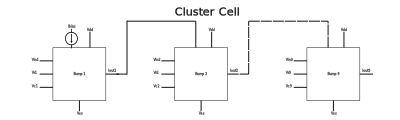
\includegraphics[width=1\columnwidth]{/home/nassosliak/Desktop/ink/cluster.png}
    \caption{Cluster circuit for 9 features}
    \label{fig:cluster}
\end{figure}
Each bump circuit includes tunable electronic components that adjust the parameters of the Gaussian distribution it represents. Specifically, the mean value of the distribution is controlled by a voltage referred to as \(V_r\), while the variance is regulated by another control voltage, \(V_{\text{control}}\). These parameters are set through a software-based training process, enabling precise adjustments based on the characteristics of the data.


The input features are provided as voltage values within each cluster cell, which are converted into output currents representing the posterior probabilities, as described in Equation 1. These output currents are then fed into a Lazzaro Winner-Take-All (WTA) circuit, which performs a function analogous to the argmax operation outlined in Equation 2. The WTA circuit allocates the entire output current to the cluster with the highest current, while setting all other cluster currents to zero. Consequently, a given sample is classified according to the cluster center with the highest probability.




\section{\textbf{Circuit Analysis}}

In this section we will be comparing two different circuits implementing the gaussian function.  A direct comparison
of both bump architectures will be
implemented, for the selection of one of them, in order to
be used in the whole system architecture. Power supply for
all circuits is set at VDD = 2.2V and VSS = 0V. Current
bias values for circuitry analysis are set at Ibias= 65nA. \\

\textbf{A. Fully tunable bulk controlled modification of Delbrucks Bump} \\
The circuit presented in Fig. 3 is a modification of the Gaussian function circuit first introduced by Delbruck in 1991 \cite{155225}. The original circuit consisted of a non-symmetric current correlator (M1–M4), a cascode differential block (M5–M6), and a current mirror (M9–M10). The modification introduces a differential pair (M7–M8) with a tunable body voltage, allowing for the adjustment of the Gaussian variance—something that the original Delbruck's Bump circuit cannot achieve. The transistor sizes for the circuit are listed in Table I.

\begin{figure}[!h]
    \centering
    \includegraphics[width=1\columnwidth]{/home/nassosliak/Desktop/ink/tundel.png}
    \caption{Fully tunable, bulk-controlled modification of
 Delbruck’s bump.}
    \label{fig:tundelfig}
\end{figure}

\begin{table}[!h]
    \centering
\large
\begin{tabular}{|p{2.5cm}|p{2.5cm}|p{2.5cm}|}
        \hline
        \textbf{Transistor} & \textbf{W/L}\\
        \hline
        M1,M4   &  wcor/1.2u\\
        \hline
         M2,M3   & 2*wcor/1.2u\\
        \hline
         M5-M8   &  wdif/1.2u\\
        \hline
         M9   & wmir/1.2u \\
        \hline
         M10   &   4*wmir/1.2u\\
        \hline
  wcor &   7.5u\\
        \hline
  wdif  &   7.5u\\
        \hline
  wmir   &   7.5u\\
        \hline
    \end{tabular}
\vspace{0.5cm}
    \caption{Sizing Parameters for Fully-Tunable Delbruck's Bump Circuit}

\end{table}
\textbf{B. Modified Bump Circuit} \\
A modified bump circuit with a symmetrical current correlator is presented in Fig. 4, which differs from the non-symmetric current correlators described in Delbruck's bump circuits \cite{155225}. This modification results in a more symmetrical Gaussian function, even for small bias currents, as demonstrated in \cite{ALIMISIS2022105510}. Furthermore, the cascode current mirror, consisting of transistors M11–M16, is employed to enhance the mirroring effect, even for small bias currents. This leads to a more robust current Gaussian function and allows for greater variability in training parameters. Sizing parameters used for the modified bump circuit can be seen in Table II.\\

\begin{figure}[!h]
    \centering
    \includegraphics[width=1\columnwidth]{/home/nassosliak/Desktop/ink/modified.png}
    \caption{Modified Bump Circuit}
\end{figure}

\begin{table}[!h]
    \centering
\large
\begin{tabular}{|p{2.5cm}|p{2.5cm}|p{2.5cm}|}
        \hline
        \textbf{Transistor} & \textbf{W/L}\\
        \hline
         M1,M4   & 4*wcor/1.2u\\
        \hline
        M2,M3,M5,M6   &  wcor/1.2u\\
        \hline
         M7,M10   &   2*wdif/1.2u\\
        \hline
         M8,M9   & wdif/1.2u \\
        \hline
         M11,M14   & wmir/1.2u \\
        \hline
         M15,M16   & 4*wmir/1.2u \\
        \hline
  wcor &   22.5u\\
        \hline
  wdif  &   63u\\
        \hline
  wmir   & 79.5u\\
        \hline

    \end{tabular}
\vspace{0.5cm}
    \caption{Sizing parameters for Modified Bump Circuit}

\end{table}

\textbf{C. Noise and PSRR comparison}
In this section, we compare the circuits described above in terms of noise and PSRR, using the previously mentioned MOS transistor sizes, power supply voltage, and bias current. As shown in Fig. 5, both circuits provide similar noise performance at low frequencies; however, the Modified Bump circuit exhibits lower noise at higher frequencies compared to Delbruck's fully tunable bump circuit. Additionally, the Modified Bump circuit achieves better PSRR values at both low and high frequencies, although it performs slightly worse in the mid-frequency range, as illustrated in Fig. 6. Based on these results, we will proceed with the Modified Bump circuit for implementing the GMM classifier. The achieved noise values and target values are presented in Table III. 

It is important to note that transistor sizing parameters and \(I_{\text{bias}}\) significantly affect noise performance. Increasing both the transistor widths and \(I_{\text{bias}}\) results in reduced noise levels.\\


\begin{figure}[!h]
    \centering
    \includegraphics[width=1\columnwidth]{/home/nassosliak/Desktop/avlsi/pictures/noise.png}
    \caption{Noise Analysis}
    \label{fig:noise}
\end{figure}

\begin{figure}[!h]
    \centering
    \includegraphics[width=1\columnwidth]{/home/nassosliak/Desktop/avlsi/pictures/psrr.png}
    \caption{PSRR Analysis}
    \label{fig:psrr}
\end{figure}


\begin{table}[!h]
    \centering
\large
\begin{tabular}{|p{2.5cm}|p{2.5cm}|p{2.5cm}|}
        \hline

        \textbf{Frequency (Hz)} & \textbf{Target Output Noise (dB)} & \textbf{Actual Output Noise (dB)} \\
        \hline
        10   & $< -92$  &-135.90 \\
        \hline
        1k   & $< -106$ & -135.90\\
        \hline
        10k  & $< -110$ & -135.90 \\
        \hline
        100k & $< -128$ & -136.60 \\
        \hline
        1M   & $< -140$ & -140.10 \\
        \hline
    \end{tabular}
\vspace{0.5cm}
    \caption{Noise Measurements}
    \label{tab:results}
\end{table}

\begin{table}[!h]
    \centering

    \begin{tabular}{|c|c|c|}
        \hline
        \textbf{Frequency (Hz)} & \textbf{Target PSRR (dB)} & \textbf{Actual PSRR (dB)} \\
        \hline
        1   & $< -36$  & -47.84 \\
        \hline
        1k   & $< -16$ & -47.81\\
        \hline
    \end{tabular}
\vspace{0.5cm}
    \caption{PSRR Measurements}
    \label{tab:psrr}
\end{table}
\textbf{D. Parametric analysis for Modified Bump Circuit}\\
To achieve high classification accuracy, several parameters must be optimized in the Modified Bump circuit, including transistor sizes and the values of \( V_c \), \( V_r \). These parameters directly affect the Gaussian function's key characteristics, such as the mean value, variance, and height \cite{electronics10202530}. By tuning these parameters, the model can achieve lower validation errors and higher accuracy due to better alignment between hardware and software training parameters.

To determine the optimal transistor sizes, parametric analysis simulations were performed with the goal of producing the desired Gaussian functions. As shown in Fig. 7, increasing the width of the differential pair transistors produces a narrower Gaussian function. Additionally, decreasing the width of the transistors in the cascode current mirror increases the height of the Gaussian function (Fig. 8), while increasing the width of the transistors in the symmetrical correlator also increases the height of the Gaussian function (Fig. 9). Moreover, as shown in Fig. 10, increasing the length of the transistors narrows the Gaussian function and increases its height up to a certain point, beyond which the height starts to decrease.

After conducting these parametric analyses and evaluating accuracy and noise performance, the final transistor sizing parameters were determined, as shown in Table II.\\

\begin{figure}[!h]
    \centering
    \includegraphics[width=0.8\columnwidth]{/home/nassosliak/Desktop/avlsi/pictures/wdif.png}
    \caption{Parametric Analysis for wdif}
    \label{fig:wdif}
\end{figure}

\begin{figure}[!h]
    \centering
    \includegraphics[width=0.8\columnwidth]{/home/nassosliak/Desktop/avlsi/pictures/wmir.png}
    \caption{Parametric Analysis for wmir}
    \label{fig:wmir}
\end{figure}

\begin{figure}[!h]
    \centering
    \includegraphics[width=0.8\columnwidth]{/home/nassosliak/Desktop/avlsi/pictures/wcor.png}
    \caption{Parametric Analysis for wcor}
    \label{fig:wcor}
\end{figure}

\begin{figure}[!h]
    \centering
    \includegraphics[width=0.8\columnwidth]{/home/nassosliak/Desktop/avlsi/pictures/l.png}
    \caption{Parametric Analysis for L}
    \label{fig:l}
\end{figure}

After defining the transistor sizing parameters for constant values of \( I_{\text{bias}} = 65 \, \text{nA} \), \( V_r = 1.4 \, \text{V} \), and \( V_c = 0 \), it is also important to conduct a parametric analysis for \( V_r \) and \( V_c \), as these voltages affect the mean and variance of the Gaussian function accordingly. As shown in Fig. 11, the value of \( V_r \) corresponds to the mean of the Gaussian function. A range of [1.25, 1.4] volts was selected for the operation of the circuit, as within this range, the height of the Gaussian function remains stable. 

Furthermore, \( V_c \) controls the variance of the Gaussian function. As shown in Fig. 12, increasing \( V_c \) increases the variance. However, \( V_c \) is not directly proportional to the variance, and to establish the relationship between variance and \( V_c \), a polynomial fit was performed using various values of \( V_c \) obtained through software training. A range of [0, 0.7] volts was chosen for \( V_c \), allowing a wide range of variances without distorting the Gaussian function. The ranges of \( I_{\text{bias}} \), \( V_c \), and \( V_r \) are summarized in Table V.\\


\begin{figure}[!h]
    \centering
    \includegraphics[width=0.8\columnwidth]{/home/nassosliak/Desktop/avlsi/pictures/vr.png}
    \caption{Parametric Analysis for Vr}
    \label{fig:vr}
\end{figure}

\begin{figure}[!h]
    \centering
    \includegraphics[width=0.8\columnwidth]{/home/nassosliak/Desktop/avlsi/pictures/vc.png}
    \caption{Parametric Analysis for Vc}
    \label{fig:vc}
\end{figure}


\begin{table}[!h]
    \centering
\large
    \begin{tabular}{|c|c|c|}
        \hline
        \textbf{Parameter} & \textbf{Min Value} & \textbf{Max Value} \\
        \hline
        Ibias   & 65n  & 65n \\
        \hline
        Vc   &  0V & 0.7V\\
        \hline
       Vr   & 1.25V & 1.4V\\
        \hline
    \end{tabular}
\vspace{0.5cm}
    \caption{Min and Max Values for Vc, Vr and Ibias}
    \label{tab:minmax}
\end{table}

\textbf{E. Lazzaro WTA Circuit}\\
A typical Lazzaro WTA (Winner-Take-All) circuit \cite{1902a535184f48ed963e5033af04007b} was used to determine the winning class, thus simulating the argmax function in hardware. The NMOS WTA circuit is shown in Fig. 13. It consists of two NMOS neuron cells, as the dataset we will evaluate the classifier with has two classes. Each neuron is responsible for the input and output of a single class, with a shared bias current, \( I_{\text{bias}} \). 

The operation of this circuit can be summarized as follows: the neuron with the maximum input current will output a positive current, while the remaining neurons will output zero current. This effectively simulates the argmax function in hardware. A test simulation, shown in Fig. 4 (\( I_{\text{bias}} = 20 \, \text{nA} \)), demonstrates this behavior: initially, when \( I_{\text{in1}} < I_{\text{in2}} \), \( I_{\text{out1}} \) is zero, and \( I_{\text{out2}} \) equals \( I_{\text{bias}} = 20 \, \text{nA} \). As \( I_{\text{in1}} \) exceeds \( I_{\text{in2}} \), the output switches, with \( I_{\text{out1}} \) taking the value of \( I_{\text{bias}} \) and \( I_{\text{out2}} \) dropping to zero. However, the transition occurs in a linear manner rather than as a step function, which may cause issues when there are multiple winners.

The sizing parameters were optimized through simulation, with a transistor width \( W = 2.25 \, \mu\text{m} \) and length \( L = 1.2 \, \mu\text{m} \), to achieve maximum classifier accuracy.

\begin{figure}[!h]
    \centering
    \includegraphics[width=0.8\columnwidth]{/home/nassosliak/Desktop/ink/wta2.png}
    \caption{Nmos Wta circuit for 2 classes}
    \label{fig:wta2}
\end{figure}

\begin{figure}[!h]
    \centering
    \includegraphics[width=0.8\columnwidth]{/home/nassosliak/Desktop/avlsi/pictures/wta.png}
    \caption{Wta Simulation}
    \label{fig:wta3}
\end{figure}



\section{\textbf{Classification and Software Comparison}}
To assess the capabilities of the GMM analog classifier, we performed a classification task using the Breast Cancer Dataset from the University of Wisconsin. This dataset includes two classes—benign and malignant—and consists of nine features. Missing values in the dataset were handled by imputing the mean value of each column. Additionally, the dataset samples were normalized using a standard scaler. The hardware system used for this task corresponds to the architecture shown in Fig.~\ref{fig:classifier}, with clusters as depicted in Fig.~\ref{fig:cluster}.

System training was conducted offline using Python software (via the Scikit-learn library). Consequently, the values for \(I_{\text{bias}}\), \(V_r\), and \(V_c\), along with the simulation time, were obtained from the software training process and subsequently used in the hardware simulations carried out in the Cadence IC Suite. The minimum and maximum values for \(V_c\), \(V_r\), and \(I_{\text{bias}}\) are presented in Table~\ref{tab:minmax}.

The results of the classification are discussed in detail in the Appendix. Remarkably, the hardware implementation achieved higher accuracy than its software counterpart as shown in Table VI. It is also noteworthy that the mean power consumption of the classifier was 45.4~µW, or 20.64~µA, which is lower than the target value of 220~µW, or 100~µA.

\begin{table}[!h]
    \centering
\large
    \begin{tabular}{|c|c|c|}
        \hline
        \textbf{Implementation} & \textbf{Accuracy} &\textbf{Required Accuracy} \\
        \hline
        Software   &  97.6\% & 87\% \\
        \hline
        Hardware   & 98.1\%  & 82\% \\
        \hline
    \end{tabular}
\vspace{0.5cm}
    \caption{Accuracy comparison}
\end{table}


\begin{figure}[!h]
    \centering
    \includegraphics[width=0.8\columnwidth]{/home/nassosliak/Desktop/avlsi/pictures/gold.png}
    \caption{Cadence classification results compared to actual results}
    \label{fig:currents}
\end{figure}



\begin{figure}[!h]
    \centering
    \includegraphics[width=0.8\columnwidth]{/home/nassosliak/Desktop/avlsi/pictures/currents.png}
    \caption{Output Currents}
    \label{fig:currents}
\end{figure}

\begin{figure}[!h]
    \centering
    \includegraphics[width=0.8\columnwidth]{/home/nassosliak/Desktop/avlsi/pictures/power.png}
    \caption{Power Consumption}
    \label{fig:power}
\end{figure}

\section{\textbf{Conclusion}}

In this work, we have demonstrated the design and implementation of a 2.2V analog Gaussian Mixture Model (GMM) classifier, highlighting its performance through the classification of the Breast Cancer Dataset. The hardware implementation not only achieved accuracy on par with its software counterpart but also slightly surpassed it, achieving an accuracy of 98.1\% compared to the software's 97.6\%. 

One of the most notable advantages of the hardware implementation is its exceptionally low power consumption. The classifier consumed only 45.4~µW, significantly lower than the target value of 220~µW, showcasing its efficiency and making it a promising candidate for future low-power machine learning applications. 

These results underscore the potential of analog integrated circuits in performing complex machine learning tasks with reduced energy consumption, paving the way for advancements in edge computing, wearable devices, and other applications where power efficiency is critical. The success of this implementation suggests that future research and development in analog hardware for machine learning could lead to even more powerful, energy-efficient technologies.

\bibliographystyle{IEEEtran}
\bibliography{references} 

\section{\textbf{Appendix}}

\begin{figure}[!h]
\Large
    \centering
    \includegraphics[width=0.8\columnwidth]{/home/nassosliak/Desktop/avlsi/pictures/cadenceconf.png}
    \caption{Cadence Confusion Matrix}
    \label{fig:cadenceconf}
\end{figure}

\begin{figure}[!h]
    \centering
    \includegraphics[width=0.8\columnwidth]{/home/nassosliak/Desktop/avlsi/pictures/cadenceclas.png}
    \caption{Cadence Classification Report}
    \label{fig:cadenceclas}
\end{figure}

\begin{figure}[!h]
    \centering
    \includegraphics[width=0.8\columnwidth]{/home/nassosliak/Desktop/avlsi/pictures/softwareconf.png}
    \caption{Software Confusion Matrix}
    \label{fig:softwareconf}
\end{figure}

\begin{figure}[!h]
    \centering
    \includegraphics[width=0.8\columnwidth]{/home/nassosliak/Desktop/avlsi/pictures/softwareclas.png}
    \caption{Software Classification Report}
    \label{fig:softwareclas}
\end{figure}
\section{\textbf{Author}}
\vspace{1cm}
\textbf{First Correspondence Author:}  
Athanasios Liakopoulos was born in Athens, Greece, in 2002 and is currently an undergraduate student at the School of Electrical \& Computer Engineering, National Technical University of Athens.  
For correspondence: nassosliak@gmail.com, +30 6955682528.

\end{document}

